% --------------------------------------------------
% --- Preamble for the reference PDF ---
% --------------------------------------------------
\documentclass[11pt]{article}
\usepackage[a4paper,left=2cm,right=2cm,top=2cm,bottom=2cm]{geometry}
\usepackage{amsmath}
\usepackage{amsthm}
\usepackage{amssymb}
\usepackage{graphicx}
\usepackage{mathtools}
\usepackage{hyperref}
\usepackage{bm}
\usepackage{enumitem}
\usepackage[dvipsnames]{xcolor}
\usepackage{ifthen}
\usepackage{helvet}
\usepackage{tikz}
\usepackage{pgfplots}
\usepackage{euler}
\pgfplotsset{compat=newest}

\renewcommand{\familydefault}{\sfdefault}
\renewcommand\thesubsection{\Roman{subsection} --}
\renewcommand\labelitemi{$\square$}
\parindent 0pt

\DeclareMathOperator\Arg{Arg}
\DeclareMathOperator\Log{Log}

%----------------------------------------------------------------------------------------
%	DEFINITIONS
%----------------------------------------------------------------------------------------

%%%%%%%%%%%%%%%%%%%%%%%%%%%%%%%%%%
% TO BE CHANGED FOR EACH STUDENT
\newcommand{\ModuleTitle}{Complex Analysis}
\newcommand{\ModuleCode}{MATH50001}
\newcommand{\AuthorCID}{01949015}
\newcommand{\Date}{\today}
\newcommand{\Assignment}{Coursework 1}
%%%%%%%%%%%%%%%%%%%%%%%%%%%%%%%%%%

% headerline definition
\newcommand{\headerline}[6]{%
	\par\medskip\noindent
	\makebox[\textwidth][s]{\rlap{\large{{\bf #1}}}\hfill\llap{\large{{\bf
						#2}}}}
	\par
	\vspace{0.5cm}
	\makebox[\textwidth][s]{\rlap{\large{{\bf CID:} #3}}\hfill} \par
	\makebox[\textwidth][s]{\rlap{\large{{\bf Date:} #4}}\hfill} \par
	\vspace{0.5cm}
	\makebox[\textwidth][c]{\large{{\bf #5}}}
	\par\medskip}

% Useful mathematical notation definitions
\def\R{\mathbb{R}}
\def\C{\mathbb{C}}
\def\0v{\mathbf{0}}
\def\uv{\mathbf{u}}
\def\vv{\mathbf{v}}
\def\wv{\mathbf{w}}
\def\rv{\mathbf{r}}
\def\pv{\mathbf{p}}
\def\av{\mathbf{a}}
\def\bv{\mathbf{b}}
\def\cv{\mathbf{c}}
\def\xv{\mathbf{x}}

\def\uvx{\hat{\bm{x}}}
\def\uvy{\hat{\bm{y}}}
\def\uvz{\hat{\bm{z}}}
\def\uvr{\hat{\bm{r}}}
\def\uvt{\hat{\bm{\theta}}}
\def\uvp{\hat{\bm{\phi}}}
\def\uvi{\hat{\mathbf{i}}}
\def\uvj{\hat{\mathbf{j}}}
\def\uvk{\hat{\mathbf{k}}}
\def\uvu{\hat{\mathbf{u}}}
\def\uvv{\hat{\mathbf{v}}}
\newcommand{\suv}[1]{\hat{\mathbf{e}}_{#1}}
\newcommand{\uuv}[1]{\mathbf{u}_{#1}}
\DeclareMathOperator{\sech}{sech}

\def\p{\partial}
\def\ux{\frac{\partial u}{\partial x}}
\def\uy{\frac{\partial u}{\partial y}}
\def\ut{\frac{\partial u}{\partial t}}
\def\uxx{\frac{\partial^2 u}{\partial x^2}}
\def\uyy{\frac{\partial^2 u}{\partial x^2}}
\def\uxy{\frac{\partial^2 u}{\partial x \partial y}}

\newcommand\underrel[3][]{\mathrel{\mathop{#3}\limits_{%
			\ifx c#1\relax\mathclap{#2}\else#2\fi}}}

%----------------------------------------------------------------------------------------
%	HYPERREFERENCES
%----------------------------------------------------------------------------------------
\PassOptionsToPackage{pdftex,hyperfootnotes=false,pdfpagelabels}{hyperref}
\usepackage{hyperref}
\pdfcompresslevel=9
\pdfadjustspacing=1

\hypersetup{
	% Uncomment the line below to remove all links (to references, figures, tables, etc)
	colorlinks=true, linktocpage=true, pdfstartpage=3, pdfstartview=FitV,
	% Uncomment the line below if you want to have black links (e.g. for printing black and white)
	%colorlinks=false, linktocpage=false, pdfborder={0 0 0}, pdfstartpage=3, pdfstartview=FitV, 
	breaklinks=true, pdfpagemode=UseNone, pageanchor=true,
	pdfpagemode=UseOutlines,
	plainpages=false, bookmarksnumbered, bookmarksopen=true,
	bookmarksopenlevel=1,
	hypertexnames=true, pdfhighlight=/O, urlcolor=MidnightBlue,
	linkcolor=NavyBlue,
	citecolor=MidnightBlue,
}
%----------------------------------------------------------------------------------------

% -----------------------------------
% --- Start of the main text ---
% -----------------------------------
\begin{document}
\newcommand{\lmr}{\fontfamily{lmr}\selectfont}
% Latin Modern Roman
\newcommand{\lmss}{\fontfamily{lmss}\selectfont}
% Latin Modern Sans
\newcommand{\lmtt}{\fontfamily{lmtt}\selectfont}
% Latin Modern Mono

% -----------------
% --- Header ---
% -----------------
\begin{minipage}{0.3\textwidth}
	
\includegraphics[width=0.85\textwidth]{Imperial_logo.pdf}
\end{minipage}
\begin{minipage}{0.7\textwidth}
	\centering
	{\sc Department of Mathematics} \\
	{\sc Imperial College London} \\
	Academic Year 2023-2024
\end{minipage}
\vspace{1em}

% --------------------------------------------
% --- Change the header line here!
\headerline{\ModuleTitle}{\ModuleCode}{\AuthorCID}{\Date}{Student Answers to
	\Assignment}
% ---------------------------------------------

% --------------------------------------------
% Start of questions
% --------------------------------------------
\begin{enumerate}

	% -----------------------------
	\item \begin{enumerate}
	\item To describe $\Omega$ we first recall $\Log(z) =
		      \ln|z|
		      + i\Arg(z)$. Since $|z| < 1$ we have
	      $\ln|z| < 0$
	      and since $\Arg(z) \in
		      (-\pi/2, \pi/2)$. The logarithm $\ln|z|$
	      can take
	      any value in $(-\infty, 0)$, therefore we're
	      looking at
	      numbers of the form $x + iy$ where $x < 0$ and $y
		      \in
		      (-\pi/2, \pi/2)$.
	      \begin{equation*}
		      f(\Omega) = \{z \in \mathbb{C} : z = x +
		      iy, x <
		      0, y \in (-\pi/2, \pi/2)\}
	      \end{equation*}
	\item Similarly, we have $|z| > 1$ so $\ln|z| > 0$ and
	      $\Arg(z) \in [0, \pi]$. The logarithm $\ln|z|$ can
	      take any value in $(0, \infty)$, therefore we're
	      looking at numbers of the form $x + iy$ where $x >
		      0$
	      and
	      $y \in [0, \pi]$.
	      \begin{equation*}
		      f(\Omega) = \{z \in \mathbb{C} : z = x +
		      iy, x >
		      0, y \in [0, \pi]\}
	      \end{equation*}

	\item We're asked to find the branch cut of the function
	      $f(z)$. This means we must find where $\Arg(\Log\frac{z-i}{z+i})$
	      jumps from $-\pi$ to $\pi$. Arguing by the definition of the
	      logarithm, this means $\Arg(\ln|\frac{z-i}{z+i}| +
		      i\Arg(\frac{z-i}{z+i}))$ must jump from
	      $-\pi$ to $\pi$

	      For $\Arg(\ln|\frac{z-i}{z+i}| + i\Arg(\frac{z-i}{z+i}))$ to be
	      $-\pi$ or $\pi$, there
	      must be no imaginary part, so $\Arg(\frac{z-i}{z+i}) = 0$, which
	      means $\frac{z-i}{z+i}$ is
	      real. This then means that the fraction cancels out as a real
	      number, so $z$ must be purely imaginary (otherwise we're met with
	      $\frac{\Re(z)
			      + \Im(z) - i + i + i}{\Re(z) + \Im(z) - i} = 1 +
		      \frac{2i}{\Re(z) + \Im(z) -
			      i}$ which can't be real if $\Re(z) \neq 0$)
	      Let $z = yi$, then we're looking at points of the form
	      $\frac{yi-i}{yi+i} = \frac{y -1}{y+1}$. For this to be negative
	      (to be in the negative real axis), we have $-1 < y < 1$. Thus, the branch cut
	      is the imaginary axis from $-i$ to $i$ exclusive.

\end{enumerate}
	      % -----------------------------
	\item \begin{enumerate}
		      \item If $|\sin(z)| \leq 1$ and $z = x + iy$ and by
		            definition of $|\sin(z)|$ we have

		            \begin{equation*}|\sin~z|=\left|\frac{1}{2i}(e^{iz}-e^{-iz})\right| \leq
			            1\end{equation*}
		            Now, we can write $e^{iz} - e^{-iz}$ as
		            $e^{i(x+iy)} -
			            e^{-i(x+iy)} = e^{ix-y} - e^{-ix+y} =
			            e^{ix}e^{-y} - e^{-ix}e^{y}$ And using
		            Euler's
		            formula

		            \begin{equation*}
			            e^{ix} = \cos(x) + i\sin(x) \quad
			            \text{and}
			            \quad
			            e^{-ix} = \cos(x) - i\sin(x)
		            \end{equation*}

		            Therefore, we have

		            \begin{equation*}
			            |\sin~z|=\left|\frac{1}{2i}((\cos(x) +
			            i\sin(x))e^{-y} - (\cos(x) -
			            i\sin(x))e^{y})\right|
		            \end{equation*}

		            \begin{equation*}
			            |\sin~z|=\left|\frac{1}{2i}(\cos(x)e^{-y} +
			            i\sin(x)e^{-y} - \cos(x)e^{y} +
			            i\sin(x)e^{y})\right|
		            \end{equation*}

		            Since $1/i = -i$ this is the same as

		            \begin{equation*}
			            |\sin~z|=\left|\frac{1}{2}(i\cos(x)(e^{y}-e^{-y})
			            + \sin(x)(e^{-y} + e^{y}))\right|
		            \end{equation*}

		            And finally

		            \begin{equation*}
			            |\sin~z|=\left|(\sin(x)\cosh(y) +
			            i\cos(x)\sinh(y))\right| =
			            \sqrt{\sin^2(x)\cosh^2(y) +
				            \cos^2(x)\sinh^2(y)}
			            \leq 1
		            \end{equation*}

		            We can simplify this if we square both sides as the
		            RHS
		            is invariant. Now, we can use
		            \begin{align*}
			            (\sin(x)\cosh(y))^{2}+(\cos(x)\sinh(y))^{2}
			             &
			            =\sin^{2}(x)(1+\sinh^{2}(y))+\cos^{2}(x)~\sinh^{2}(y) \\
			             &
			            =\sin^{2}(x)+(\sin^{2}(x)+\cos^{2}(x))\sinh^{2}(y)    \\
			             & =\sin^{2}(x)+\sinh^{2}(y)
			            \\
		            \end{align*}

		            Therefore, we are looking at the complex numbers $z
			            = x
			            + iy$ such that
		            \begin{equation}\sin^{2}(x)+\sinh^{2}(y) \leq
			            1\end{equation}

		            The region described by this inequality can be
		            visualized in Figure~\ref{fig:1a}.
		            \begin{figure}[h]
			            \centering

			            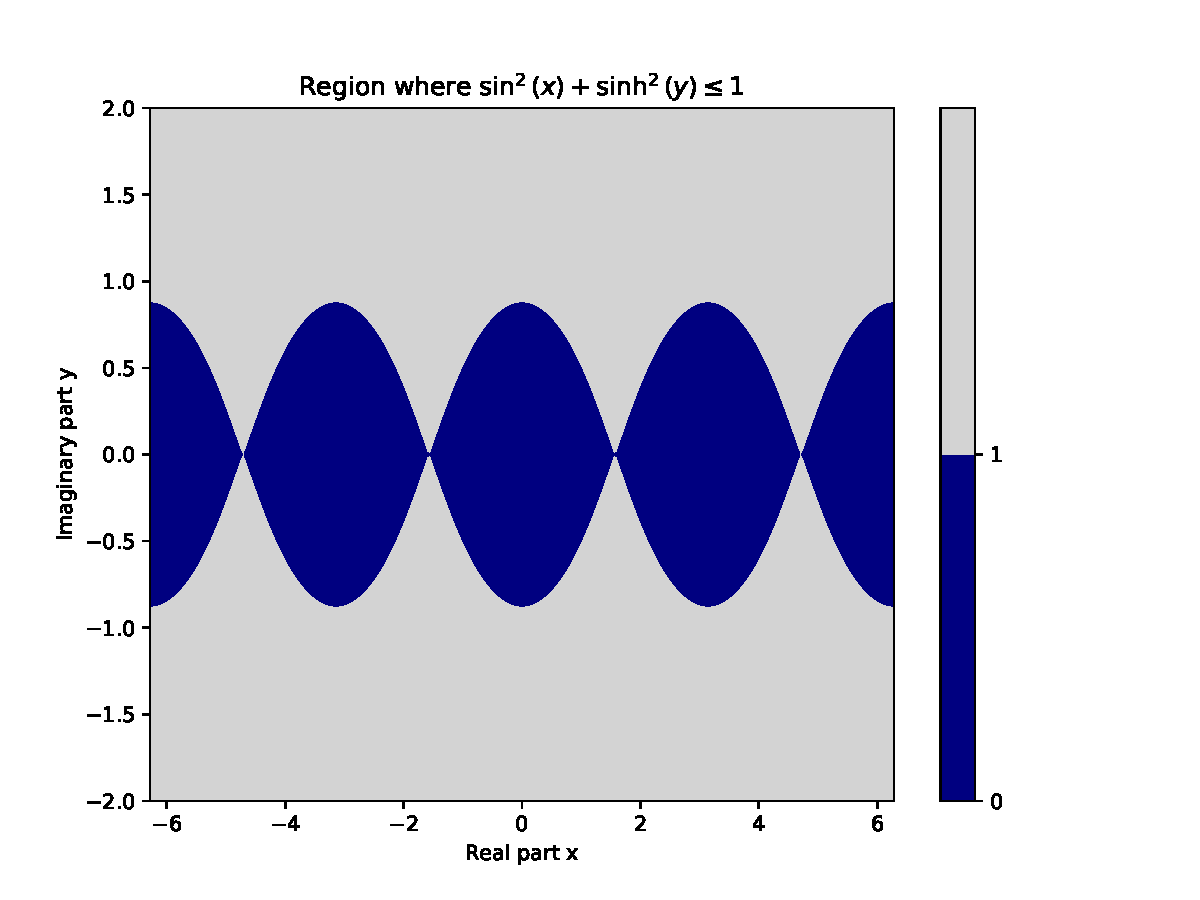
\includegraphics[width=0.5\textwidth]{sinz.pdf}
			            \caption{The region described by the
				            inequality
				            $\sin^{2}(x)+\sinh^{2}(y) \leq 1$}
			            \label{fig:1a}
		            \end{figure}

		      \item Let's find Taylor series for $f =
	\frac{1}{(z+i)(z-2)}$. First, recall

\begin{equation}\label{eq:taylor}
	f_{z_0}(z) = \sum_{n=0}^{\infty}
	\frac{f^{(n)}(z_0)}{n!} (z-z_0)^n
\end{equation}

We're asked to set $z_0 = 1$. Notice that since
$(z+i)(z-2)$ is entire, $1$ is entire and the
denominator is not 0 at $z_0 = 1$
and thus $f$ is holomorphic at $z_0 = 1$.

We can already see that the derivatives will be too
complicated to compute. Let's try to simplify the
function first. We can use
partial fractions to write $f$ as a sum of two
simpler functions:

\begin{equation}
	f(z) = \frac{1}{(z+i)(z-2)} = \frac{A}{z+i}
	+ \frac{B}{z-2}
\end{equation}

Multiplying both sides by $(z+i)(z-2)$
we get $1 = A(z-2) + B(z+i)$. We can solve for $A$
and $B$ by setting $z = -i$
and $z = 2$:

And so, $1 = (-i-2)A$ and $1 = (2+i)B$. Solving we get $A = \frac{1}{-i-2}$
and $B = \frac{1}{i+2}$. Now, the simplification leads to:

\begin{align*}
	 & B = \frac{1}{i+2}\frac{i-2}{i-2} = \frac{i-2}{-5} = \frac{2}{5} - \frac{i}{5}      \\
	 & A = \frac{1}{-i-2}\frac{-i+2}{-i+2} = \frac{-i+2}{-5} = \frac{-2}{5} + \frac{i}{5}
\end{align*}

Let $\kappa = -\frac{2}{5} + \frac{i}{5}$. Then we have:

\begin{equation}
	f(z) = \frac{1}{(z+i)(z-2)} = \kappa\left(\frac{1}{z+i} - \frac{1}{z-2}\right)
\end{equation}

And now, calculating derivatives becomes much easier:

\begin{align*}
	 & f'(z)   = \kappa\left(-\frac{1}{(z+i)^2} + \frac{1}{(z-2)^2}\right)                        \\
	 & f''(z)  = \kappa\left(\frac{2}{(z+i)^3} - \frac{2}{(z-2)^3}\right)                         \\
	 & f'''(z) = \kappa\left(-\frac{6}{(z+i)^4} + \frac{6}{(z-2)^4}\right)                        \\
	 & \cdots                                                                                     \\
	 & f^{(n)}(z) = (-1)^{n} \kappa n! \left(\frac{1}{(z+i)^{n+1}} - \frac{1}{(z-2)^{n+1}}\right)
\end{align*}

And, applying this to $z_0 = 1$, we get:

\begin{equation}\label{eq:derivative_for_n}
    f^{(n)}(1) =  \kappa n! \left(\frac{(-1)^{n}}{(1+i)^{n+1}} + 1\right)
\end{equation}

Now, plugging~\eqref{eq:derivative_for_n} into~\eqref{eq:taylor} we get:

\begin{equation}\label{eq:taylor_series}
	f_{z_0}(z) = \kappa \sum_{n=0}^{\infty}
	\left(\frac{(-1)^{n}}{(1+i)^{n+1}} + 1\right) (z-1)^n
\end{equation}

Where $\kappa = -\frac{2}{5} + \frac{i}{5}$.


	      \end{enumerate}
	      % -----------------------------
	\item \begin{enumerate}
		      \item We are asked to find the value of the integral
$\oint_{\gamma}\left(\frac{3}{z+2}-\frac{1}{z-2i}\right)dz$ along the curve
$\gamma$ given by $\{|z|=5\}$. We can split the integral into two parts:

\begin{align*}
    \oint_{\gamma}\left(\frac{3}{z+2}-\frac{1}{z-2i}\right)dz & =
    \oint_{\gamma}\frac{3}{z+2}dz - \oint_{\gamma}\frac{1}{z-2i}dz
\end{align*}

And evaluate them separately. Since $2i$ and $-2$ are inside the curve
$\gamma$, and $f(z) = c$ is entire for any constant $c$, we can use Cauchy's
integral formula to evaluate the integrals. Recall Cauchy's integral formula:

\begin{align*}
    f(z_0) & = \frac{1}{2\pi i}\oint_{\gamma}\frac{f(z)}{z-z_0}dz
\end{align*}

Which gives us the value of the integral as $2\pi i f(z_0)$. We can rewrite the integral as

\begin{align*}
    \oint_{\gamma}\frac{3}{z+2}dz & = 3\oint_{\gamma}\frac{1}{z+2}dz = 3\cdot 2\pi i = 6\pi i
\end{align*}

The same goes for the second integral:

\begin{align*}
    \oint_{\gamma}\frac{1}{z-2i}dz & = 2\pi i
\end{align*}

And now, we can add them together to get the value of the original integral:

\begin{align*}
    \oint_{\gamma}\left(\frac{3}{z+2}-\frac{1}{z-2i}\right)dz & = 6\pi i - 2\pi i = 4\pi i
\end{align*}
		      \item Similarly, we're asked for the same integral, but this time along the curve
$\gamma$ given by $\{|z - 2i| = 1/2\}$.

\begin{align*}
    \oint_{\gamma}\left(\frac{3}{z+2}-\frac{1}{z-2i}\right)dz & =
    \oint_{\gamma}\frac{3}{z+2}dz - \oint_{\gamma}\frac{1}{z-2i}dz
\end{align*}

If we call $f_1(z) = 3/(z+2)$ and $f_2(z) = 1/(z-2i)$, we know that $f_1(z)$ is
holomorphic in the disc $|z - 2i| \leq 1/2$. Thus, by the Cauchy-Goursat
theorem for discs:

\begin{align*}
    \oint_{\gamma}\frac{3}{z+2}dz & = 0
\end{align*}

This leaves the second integral as the only one to evaluate. Proceeding with
Cauchy's formula as before:

\begin{align*}
    \oint_{\gamma}\frac{1}{z-2i}dz & = 2\pi i
\end{align*}

So, this leaves

\begin{align*}
    \oint_{\gamma}\left(\frac{3}{z+2}-\frac{1}{z-2i}\right)dz & = 0 - 2\pi i = -2\pi i
\end{align*}
		      \item Take the figure eight curve. We can split it into two curves cutting by the
intersection point, and then consider both curves separately. Traversing one of
the curves in any direction means we traverse the other in opposite direction.
By the deformation theorem, this reduces to calculating the integral caused by
the singularities at the interiors of both curves. Let's call the function
we're integrating $f(z)$. We can write the integral as

\[ \oint_\gamma \frac{{8z - 3}}{{z^2 - z}}  dz = \oint_\gamma f(z) dz\]

For the region on the left, denoted as $\gamma_1$, we can express $f(z)$ as:

\[ f(z) = \frac{{8z - 3}}{{z^2 - z}} = \frac{\frac{8z - 3}{z-1}}{{z}}\]

If we call $g_1(z) = \frac{8z - 3}{z-1}$, we can see that $g(z)$ is holomorphic
in the left region because it's the division of two entire functions and the
denominator is not 0 in this region. Thus, we can apply the Cauchy formula once
again.

\begin{align*}
    2\pi ig_1(z_0) & = \oint_{\gamma_1}\frac{g_1(z)}{z-z_0}dz
\end{align*}

Since $g_1(0) = 3$, $\oint_{\gamma_1}\frac{g(z)}{z-z_0}dz = 6\pi i$.

By a similar argument, call the right region $\gamma_2$ and $g_2(z) = \frac{8z
        - 3}{z}$, and we can see that $g(1) = 5$, so
$\oint_{\gamma_2}\frac{g(z)}{z-z_0}dz = 10\pi i$. Since we traverse the left
curve in the positive direction and the right curve in the negative direction,
we can add the two integrals together to get the value of the original
integral:

\begin{align*}
    \oint_\gamma \frac{{8z - 3}}{{z^2 - z}}  dz & = 6\pi i - 10\pi i = -4\pi i
\end{align*}
	      \end{enumerate}
	\item Since $f$ is entire, we can consider its MacLaurin series:
	      \begin{equation*}
		      f(z) = \sum_{n=0}^{\infty} \frac{f^{(n)}(0)}{n!} z^n =
		      a_0 +
		      a_1z +
		      a_2z^2 + \ldots
	      \end{equation*}
	      Where $a_i$ is the complex coefficient of $z^i$ in the MacLaurin
	      expansion. Assume $a_i \neq 0$ for $i \geq 2$, then $|f(z)| = a_0
		      +
		      a_1z +
		      a_2z^2 + \ldots$, so the limit becomes

	      \begin{equation*}
		      \lim_{|z| \to \infty}\frac{|f(z)|}{|z|^2} = \lim_{|z| \to
			      \infty}\frac{|a_0 + a_1z +
			      a_2z^2 + \ldots|}{|z|^2} = \lim_{|z| \to
			      \infty}\left|\frac{a_0 + a_1z +
			      a_2z^2 + \ldots}{z^2}\right|
	      \end{equation*}

	      Applying the division, we get:

	      \begin{equation*}
		      \lim_{|z| \to \infty}\left|\frac{a_0 + a_1z +
			      a_2z^2 + \ldots}{z^2}\right| = \lim_{|z| \to
			      \infty}\left|\frac{a_0}{z^2} + \frac{a_1}{z} +
		      a_2 + \ldots\right| = 0
	      \end{equation*}

	      This is true if and only if the complex number tends to 0, so we
	      have:

	      \begin{equation*}
		      \lim_{|z| \to \infty}\frac{a_0}{z^2} + \frac{a_1}{z} +
		      a_2 + \cdots = 0
	      \end{equation*}

	      And since the limit of the sum is the sum of the limits:

	      \begin{equation*}
		      \lim_{|z| \to \infty}\frac{a_0}{z^2} + \lim_{|z| \to
			      \infty}\frac{a_1}{z} +
		      \lim_{|z| \to \infty}a_2 + \cdots = 0
	      \end{equation*}

	      And we know that $\lim_{|z| \to
			      \infty}\left|\frac{a_0}{z^2}\right|
		      = 0$ and $\lim_{|z| \to \infty}\left|\frac{a_1}{z}\right|
		      =
		      0$, because $a_0$
	      and $a_1$ are constants. Once again, since the modulus is 0, the
	      number must be 0, so the limit becomes:

	      \begin{equation*}
		      \lim_{|z| \to \infty}a_2 + \lim_{|z| \to \infty}a_3z +
		      \cdots
		      = a_2 + \lim_{|z| \to \infty}\sum_{n=3}^{\infty}a_n
		      z^{n-2} =
		      0
	      \end{equation*}

	      So the limit of the sum is $-a_2$, like so:

	      \begin{equation*}
		      \lim_{|z| \to \infty}\sum_{n=3}^{\infty}a_n z^{n-2} =
		      -a_2
	      \end{equation*}

	      Taking the modulus of both sides, we get:

	      \begin{equation*}
		      \lim_{|z| \to \infty}\left|\sum_{n=3}^{\infty}a_n
		      z^{n-2}\right|
		      = |-a_2| = |a_2|
	      \end{equation*}

	      Since the LHS doesn't have singularities, and the limit is
	      finite,
	      we can bound the sum by a constant $M$:

	      \begin{equation*}
		      \left|\sum_{n=3}^{\infty}a_n z^{n-2}\right| \leq M
	      \end{equation*}

	      But, by Liouville's theorem ($*$), if $s(z) =
		      \sum_{n=3}^{\infty}a_n
		      z^{n-2}$ is
	      bounded, then it is constant. Since the
	      limit is $-a_2$, then

	      \begin{equation*}
		      s(z) = \sum_{n=3}^{\infty}a_n z^{n-2} = -a_2
	      \end{equation*}

	      But since $s(0) = 0$, then $-a_2 = 0$, so $a_2 = 0$, and $s(z) =
		      \sum_{n=3}^{\infty}a_n z^{n-2} = 0$

	      Going back to the Maclaurin expansion of $f$, we have:

	      \begin{equation*}
		      f(z) = a_0 + a_1z + a_2z^2 + z^2\sum_{n=3}^{\infty}a_n
		      z^{n-2} = a_0 + a_1z
	      \end{equation*}

	      If we rename $a_0 = a$ and $a_1 = b$, we get the final result:

	      \begin{align*}
		      f(z) = a + bz \\ a, b \in \mathbb{C}
	      \end{align*}

	      ($*$) Here we need to be careful as $s(z)$
	      was obtained by $\frac{f(z)-a_2z^2-a_1z-a_0}{z^2}$, so we would
	      really be
	      talking about a function which takes this fraction in $\C -
		      \{0\}$
	      and $0$
	      if $z = 0$, and this function is holomorphic at $\C - \{0\}$, but
	      we need to check that it is also holomorphic at $0$ to make sure
	      that we can apply the
	      theorem. Following the actual piecewise definition of $s(z)$

	      \begin{equation*}
		      s(z) = \begin{cases}
			      \frac{f(z)-a_2z^2-a_1z-a_0}{z^2} & \text{if } z
			      \neq 0
			      \\
			      0                                & \text{if } z =
			      0
		      \end{cases}
	      \end{equation*}

	      To check whether $s(z)$ is holomorphic at $0$, we need to check
	      if

	      \begin{equation*}
		      \lim_{h \to 0}\frac{s(h) - s(0)}{h-0} = \lim_{h \to
			      0}\frac{s(h)}{h}
	      \end{equation*}

	      converges.
	      Note $f(h) - a_2h^2 - a_1h - a_0 = h^2\sum_{n=3}^\infty a_n
		      h^{n-2}$, so

	      \begin{equation*}
		      \lim_{h \to 0}\frac{s(h)}{h} = \lim_{h \to
			      0}\frac{h^2\sum_{n=3}^\infty a_n h^{n-2}}{h^2} =
		      \lim_{h \to
			      0}\sum_{n=3}^\infty a_n h^{n-3} = a_3
	      \end{equation*}

	      So $s(z)$ is holomorphic at $0$, and thus it is entire.

\end{enumerate}

\end{document}
